\chapter{The DUNE Near Detector} % Executive Summary}
\label{ch:exsum-nd}

\textit{This chapter briefly introduces the DUNE near detector, emphasizing its role for the DUNE far detector physics program.  More details on the near detector may be found in  appendices of this TDR volume.  DUNE will issue a complete conceptual design report for the near detector in late 2019, with a technical design report to follow in 2020.}

%%%%%%%%%%%%%%%%%%%%%%%%%%%%%%%%%%%%%%%%%%%%%%%%%%%%%%%%%%%%%%
\section{Overview of the DUNE Near Detector}
\label{sec:exsum-nd-overview}


\subsection{Motivation}
\label{sec:exsum-nd-BriefOverview-need}

%This chapter briefly summarizes the purpose and reference design concept for the \dword{dune} \dword{nd}.  A more complete description may be found in the appendices of this volume.

The \dword{dune} experiment will measure oscillation probabilities for muon neutrinos or antineutrinos to either remain the same flavor or oscillate into their electron flavor counterparts as a function of the neutrino energy. This will allow the neutrino mass ordering to be definitively determined, as well as enable observation of leptonic \dword{cpv} for a significant range of $\delta_{\rm{CP}}$ values and precise measurement of % \dword{pmns}
neutrino mixing matrix parameters.

The \dword{nd} will serve as the experiment's control,
 constraining systematic errors and measuring the initial unoscillated \numu and \nue energy spectra (and that of the corresponding antineutrinos). 
 The energy spectra result from an energy-dependent convolution of flux, cross section, and detector response for each of the four %(two-flavor, (anti)neutrino) 
 neutrino types (\nue, \numu, \anue, \anumu). 
  The \dword{nd} will make measurements that allow the three functions to be independently constrained and partially or fully deconvolved. The constraints will be used to improve the simulation program that is responsible for predicting the energy spectra at the \dword{fd} for particular choices of the oscillation parameters. This allows the actual oscillation parameters to be estimated from a fit to the \dword{fd} data. 
 

The \dword{nd} will also have a physics program of its own, independent of the far detector.  This program will include measuring neutrino interactions to explore the two pillars of the standard model: electroweak physics and quantum chromodynamics. The \dword{nd} physics program will also explore physics beyond the standard model. This includes searches for non-standard interactions, sterile neutrinos,  dark photons, and  other exotic particles.

 %%%%%%%%%%%%%%%%%%%%%%%%%
\subsection{Requirements}
\label{sec:exsum-nd-requirements}

The components of the  \dword{nd} must address their multiple missions in a complementary fashion. In this section, we list the key overarching requirements driving the \dword{nd} complex. Section~\ref{sec:appx-nd:requirements} in Appendix~\ref{ch:appx-nd} goes into more detail, discussing some thought experiments and case studies that illustrate how different parts of the complex work together. These case studies naturally suggest more detailed capabilities, performance statistics, and technical requirements; we are in the process of tabulating them. 

\begin{itemize}
    \item  \textit{Predict the neutrino spectrum at the \dword{fd}} The \dword{nd} must predict the energy spectrum of \numu, \anumu, \nue and \anue at the \dword{fd}. The prediction must be provided as a function of the oscillation parameters, and systematic uncertainties must be small enough to achieve the required \dword{cp} coverage. This is the primary requirement of the \dword{dune} \dword{nd}.
    
    \item \textit{Measure interactions on argon} The \dword{nd} must measure neutrino interactions on argon to reduce uncertainties due to nuclear modeling. The \dword{nd} must be able to determine the neutrino flavor and measure the full kinematic range of the interactions that will be seen at the \dword{fd}.
    
    \item \textit{Measure the neutrino energy} The \dword{nd} must be able to reconstruct the neutrino energy in \dword{cc} events and control for any biases in energy scale or resolution, keeping them small enough to achieve the required \dword{cp} coverage. These measurements must also be transferable to the \dword{fd}. 
    
    \item \textit{Constrain the cross section model} The \dword{nd} must measure neutrino cross sections in order to constrain the cross section model used in the oscillation analysis. In particular, cross section mismodeling that causes incorrect \dword{fd} predictions as a function of neutrino flavor and true or reconstructed energy must be constrained well enough to achieve the required \dword{cp} coverage. 
    
    \item \textit{Measure neutrino fluxes} The \dword{nd} must measure neutrino fluxes as a function of flavor and neutrino energy. This allows neutrino cross section to be measured and constrains the beam model and the extrapolation of neutrino energy spectra from the \dword{nd} to the \dword{fd}.
    
    \item \textit{Obtain data with different fluxes} The \dword{nd} must measure neutrino interactions in different beam fluxes (especially ones with different mean energies) to disentangle flux and cross sections, verify the beam model, and guard against systematic uncertainties on the neutrino energy reconstruction.
    
    \item \textit{Monitor the neutrino beam} The \dword{nd} must monitor the neutrino beam energy spectrum with sufficient statistics to be sensitive to intentional or accidental changes in the beam on short timescales. The precise requirement will be informed by the run plan and by experience from previous experiments. 
    
\end{itemize}


\subsection{Design}
\label{sec:exsum-nd-BriefOverview-design}


The \dword{dune} \dword{nd} is formed from three primary detector components and the capability of two of those components to move off the beam axis. The three detector components serve important individual and overlapping functions in the \dword{nd} mission.  Because these components have standalone features, the \dword{dune} \dword{nd} is often discussed as a suite or complex of detectors and capabilities.  The movement off axis provides a valuable extra degree of freedom in the data, which is discussed extensively in this report.  The power in the \dword{dune} \dword{nd} concept lies in the collective set of capabilities.  

The \dword{dune} \dword{nd} is shown in the \dword{dune} \dword{nd} hall in Figure~\ref{fig:es:NDHallconfigs}.  Table~\ref{tab:NDsummch} provides a high-level overview of the three components of the \dword{dune} \dword{nd} along with the off-axis capability that is sometimes described as a fourth component.  

\begin{dunefigure}[DUNE near detector hall with component detectors]{fig:es:NDHallconfigs}
{\dword{dune} \dword{nd} hall shown with component detectors, all in the on-axis configuration (left) and with the \dword{lartpc} and \dword{mpd} in an off-axis configuration (right). The \dword{3dsts}, consisting of the \dword{3dst}  inside the \dword{kloe} magnet is shown in position on the beam axis. The beam enters the hall at the bottom of the drawings moving from right to left.}
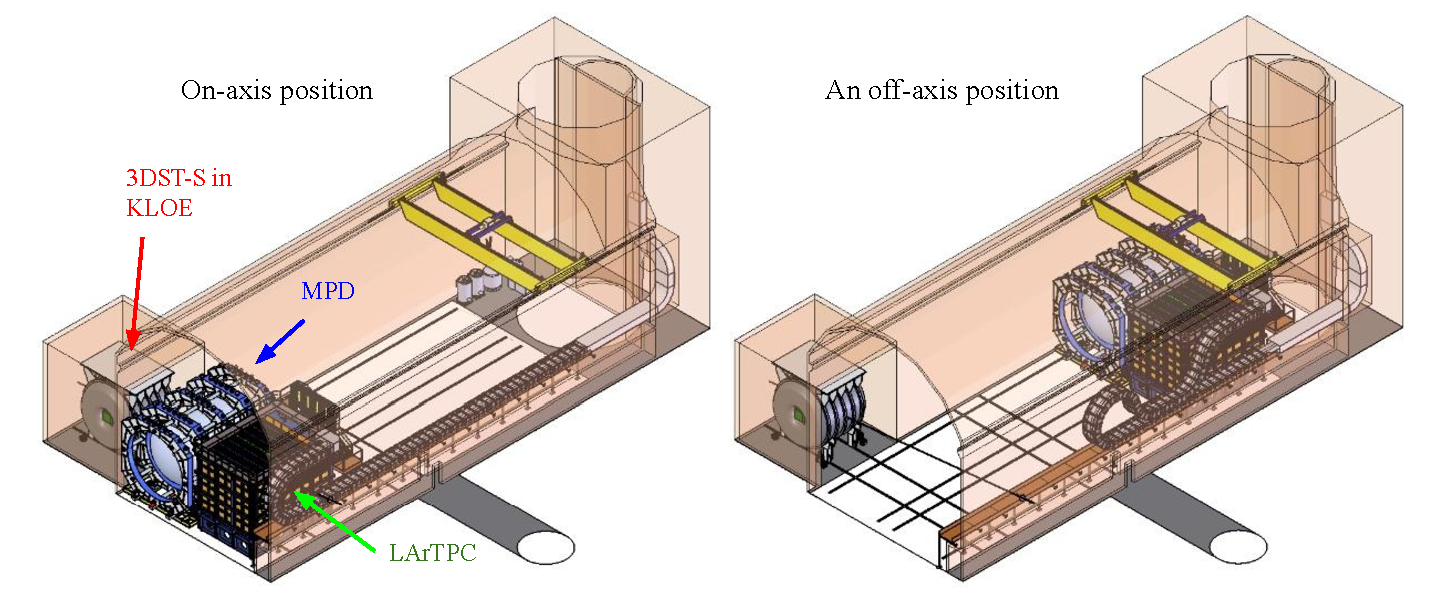
\includegraphics[width=\textwidth]{graphics/hall_drawing_oct_19.pdf}
\end{dunefigure}



\begin{dunetable}[Components of the DUNE ND]
{p{.22\textwidth}p{.22\textwidth}p{.22\textwidth}p{.22\textwidth}}
{tab:NDsummch}{This table gives a high-level breakdown of the three major detector components and the capability of movement for the DUNE ND along with function and primary physics goals.}
Component & Essential Characteristics & Primary function & Select physics aims \\ \toprowrule
LArTPC (ArgonCube) & Mass  & Experimental control for the Far Detector & $\numu$($\overline{\nu}_{\mu}$) CC \\
          & Target nucleus Ar &  Measure unoscillated $E_\nu$ spectra   & $\nu$-e$^{-}$ scattering   \\
          &  Technology FD-like    &  Flux determination  &  $\nue +$$\overline{\nu}_{e}$ CC  \\
          &  &  &  Interaction model \\ \colhline
Multipurpose detector (MPD) & Magnetic field & Experimental control for the LArTPCs & $\numu$($\overline{\nu}_{\mu}$) CC \\
  &  Target nucleus Ar & Momentum analyze liquid Ar $\mu$ & $\nue$ CC, $\overline{\nu}_{e}$ \\
  & Low density & Measure exclusive final states with low momentum threshold & Interaction model \\  \colhline
DUNE-PRISM (capability) & LArTPC$+$MPD move off-axis & Change flux spectrum &  Deconvolve flux $\times$ cross section \\ 
 & & & Energy reponse \\
 & & & Provide FD-like energy spectrum at ND\\ 
% & & & {\   }differences \\
 & & & ID mismodeling \\ \colhline
%\dword{3dsts} 
Beam Monitor (\dshort{3dsts}) & On-axis & Beam flux monitor &  On-axis flux stability \\ 
  & High mass CH target & Neutrons & Interaction model \\ 
& KLOE magnet &  & A dependence \\
    &  & & $\nu$-e$^{-}$ scattering \\ 
\end{dunetable}



The core part of the \dword{dune} \dword{nd} is a \dword{lartpc} called \dword{arcube}.  \dword{arcube} consists of an array of 35 modular \dwords{tpc} sharing a cryostat.  A drawing of a prototype of the modular \dwords{tpc} is illustrated in Figure~\ref{fig:es:ac_module}.  
This detector has the same target nucleus and shares some aspects of form and functionality with the \dword{fd}, where the differences are necessitated by the expected intensity of the beam at the \dword{nd}.  This similarity in target nucleus and technology reduces sensitivity to nuclear effects and detector-driven systematic errors in the extraction of the oscillation signal at the  \dword{fd}.  The \dword{lartpc} is large enough to provide high statistics %($\num{1e8}{\numu \text{-CC events/year}}$) 
($\num{e8}{\numu \text{-CC events/year}}$) and sufficient volume to provide good hadron containment.  The tracking and energy resolution, combined with the mass of the \dword{lartpc}, will allow the flux in the beam to be measured using several techniques, including the well understood but rare process of $\numu$-e$^{-}$ scattering.

\begin{dunefigure}[ArgonCube 2$\times$2 demonstrator module]{fig:es:ac_module}
{Cutaway drawing of a \SI{0.67 x 0.67 x 1.81}{\metre} \dword{arcube} prototype module. For illustrative purposes, the drawing shows traditional field shaping rings instead of a resistive field shell. Note the G10 walls will completely seal the module, isolating it from the neighboring modules and the outer \dword{lar} bath. Also note the modules in this prototype system will not have individual pumps and filters.}
\includegraphics[width=0.8\textwidth]{graphics/Normal-Module-4K_labelled.jpeg}
\end{dunefigure}

The \dword{lartpc} begins to lose acceptance for muons above 0.7 GeV/c momentum due to lack of containment.  Because the muon momentum is a critical component of the neutrino energy determination, a magnetic spectrometer is needed downstream of the \dword{lartpc} to measure the charge sign and momentum of these muons.  This function is accomplished by the multipurpose detector (\dword{mpd}), which consists of a high-pressure gaseous argon \dword{tpc} (\dword{hpgtpc}) surrounded by an \dword{ecal} in a \SI{0.5}{T} magnetic field (Figures~\ref{fig:es:ConceptDesign_NDECAL} and~\ref{fig:es:ConceptTile_NDECAL}). 
The \dword{hpgtpc} provides a lower density medium with excellent tracking resolution for the muons from the \dword{lartpc}.  In addition, with this choice of technology for the tracker, neutrinos interacting on the argon in the gas \dword{tpc} constitute a sample of $\nu$-Ar events that can be studied with a very low charged particle tracking threshold, excellent kinematic resolution, and systematic errors that differ from the liquid detector. The high pressure results in a sample of $\num{2e6}$ ${\numu \text{-CC events/year}}$ for these studies. These events will be valuable for studying the charged particle activity near the interaction vertex because this detector can access lower momentum protons than the \dword{lar} detector and has better particle identification of charged pions.  The relative reduction in secondary interactions in these samples (compared to \dword{lar}) will help in identifying the particles produced in the primary interaction and modeling secondary interactions in denser detectors, which are known to be important \cite{Friedland:2018vry}.
In addition, many neutrons produced in neutrino interactions in the gaseous argon may be reconstructed via time-of-flight using the \dword{ecal}.    
  
%The \dword{mpd} is  discussed further in Section~\ref{ssec:exsum-nd-mpd}.

\begin{dunefigure}[\dshort{mpd} ECAL conceptual design]{fig:es:ConceptDesign_NDECAL}
{The conceptual design of the MPD system for the \dword{nd}. The TPC is shown in yellow inside the pressure vessel.  Outside the pressure vessel, the \dword{ecal} is shown in organge, and outside that are the magnet coils and cryostats.  The drawing illustrates the five-coil superconducting design.}
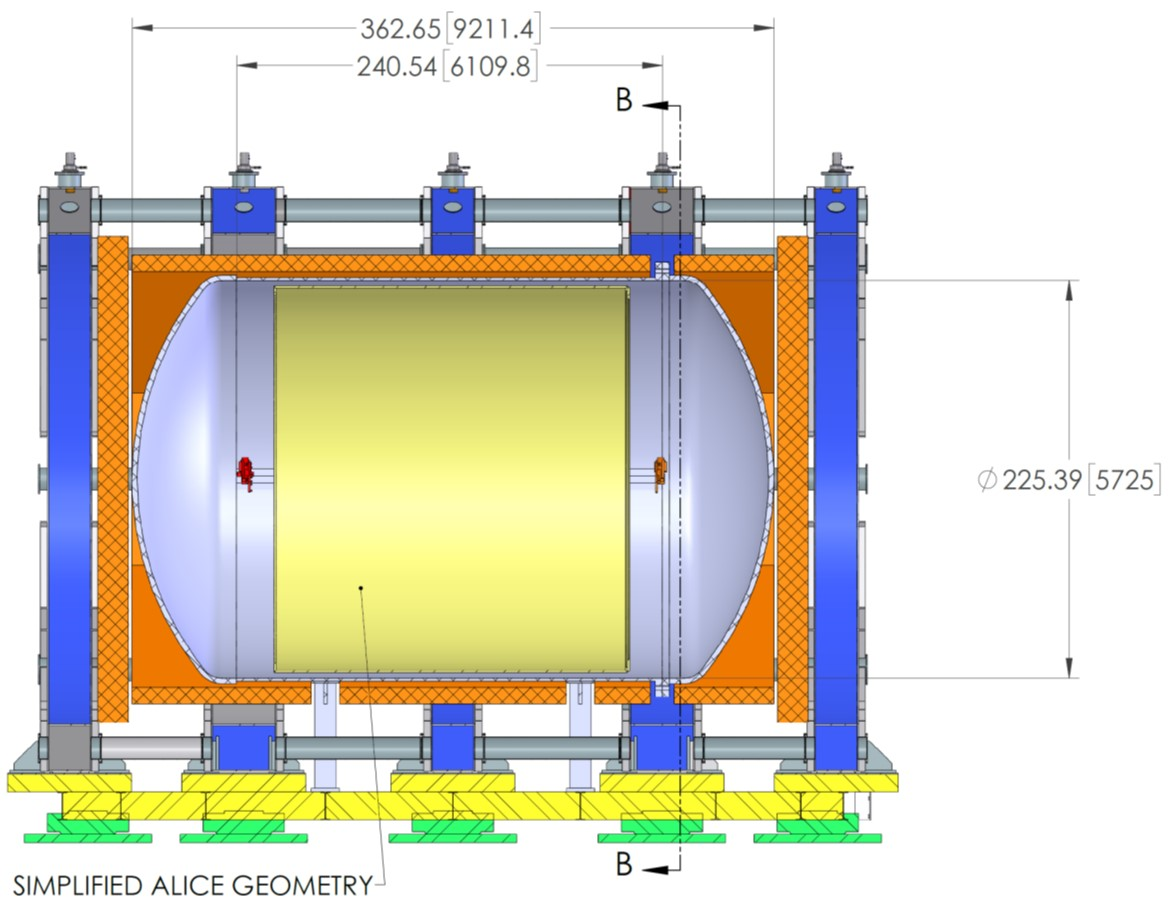
\includegraphics[width=0.8\textwidth]{graphics/MPDdrawing.jpg}
%\includegraphics[width=0.42\textwidth]{graphics/ECAL_Endcap_System.png}
\end{dunefigure}

\begin{dunefigure}[Conceptual layout of the \dshort{mpd} ECAL]{fig:es:ConceptTile_NDECAL}
{Conceptual layout of the calorimeter showing the absorber structure, scintillator tiles, \dword{sipm}, and \dword{pcb}. The scintillating layers consist of a mix of tiles and cross-strips with embedded wavelength shifting fibers to achieve a comparable effective granularity.}
\includegraphics[width=0.8\textwidth]{graphics/TileConcept.png}
\end{dunefigure}

The \dword{lartpc} and \dword{mpd} can move to take data in positions off the beam axis.  This capability is referred to as \dword{duneprism}. As the detectors move off-axis, the incident neutrino flux spectrum changes, with the mean energy dropping and the spectrum becoming more monochromatic.  Though the neutrino interaction rate drops off-axis, the intensity of the beam and the size of the \dword{lartpc}  combine to yield ample statistics even in the off-axis positions. 
Figure~\ref{fig:es:offaxisfluxes} shows a sample of neutrino energy distributions taken at different off-axis angles.
%
Data taken at different off-axis angles allows the deconvolution of the neutrino flux and interaction cross section and mapping of the reconstructed versus true energy response of the detector.  This latter mapping is applicable at the \dword{fd} up to the level to which the near and far \dword{lar} detectors are similar.  Stated a different way, it is possible to use information from a linear combination of the different fluxes to create a data sample at the \dword{nd} with an effective neutrino energy distribution close to the oscillated spectrum at the \dword{fd}.  This data-driven technique will reduce systematic effects coming from differences in the energy spectra of the oscillated signal events in the \dword{fd} and the \dword{nd} samples used to constrain the interaction model. Finally, the off-axis degree of freedom provides a sensitivity to some forms of mismodeling in the beam and/or interaction models. %The \dword{duneprism} program is discussed further in Section~\ref{sec:exsum-nd-DP}. 

Figure~\ref{fig:es:duneprismfluxfits} shows linear combinations of off-axis fluxes giving \dword{fd} oscillated spectra for two sets of oscillation parameters. The procedure can model the \dword{fd} flux well for neutrino energies in the range of 0.6-3.6~GeV. The input spectra for the linear combinations, shown in Figure~\ref{fig:es:offaxisfluxes}, extend only slightly outside this range and cannot be combined in a linear fashion to model well the flux outside that range. The modeled range encompasses the range of data of interest for the oscillation program.   


%\fixme{This shows up in the PDF as an incomplete sentence. What shows?}

%%%
\begin{dunefigure}[Variation of neutrino energy spectrum as function of off-axis angle]{fig:es:offaxisfluxes}
{The variation in the neutrino energy spectrum shown as a function of detector off-axis position, assuming the nominal \dword{nd} location 574~m downstream from the production target.}
\includegraphics[width=0.8\textwidth]{offaxisfluxes.pdf}
\end{dunefigure}
%%
\begin{dunefigure}[Linear combinations of off-axis fluxes giving FD oscillated spectra]{fig:es:duneprismfluxfits}
{Linear combinations of off-axis fluxes giving \dword{fd} oscillated spectra for a range of oscillation parameters. The  \dword{fd} oscillated flux is shown in black, the target flux is shown in green, and the linearly combined flux obtained with the nominal beam \dword{mc} is shown in red. Systematic effects due to 1$\,\sigma$ variations of the decay pipe radius (green), horn current (magenta), and horn cooling water layer thickness (teal) are also shown.}
	\includegraphics[width=0.7\textwidth]{nuprism_coef_oscSpectrum_0_0022_0_5.pdf}
	\includegraphics[width=0.7\textwidth]{nuprism_coef_oscSpectrum_0_0025_0_65.pdf}
\end{dunefigure}
%%

The final component of the \dword{dune} \dword{nd} suite is the beam monitor, %\threed projection scintillator tracker spectrometer (\dword{3dsts}),  
the core part of which is the \dword{3dst} mounted within the KLOE magnet and calorimeter, as illustrated in Figure~\ref{fig:es:3dst-geometry}.  The \dword{3dst} is a plastic scintillator detector made of \SI{1}{\cubic\centi\meter} cubes read out along each of three orthogonal dimensions.  The design eliminates the typical planar-strip geometry common to detectors using a scintillator, leading to improved acceptance at large angles relative to the beam direction.  The \dword{3dst} is situated along the beam axis inside an envelope of high resolution, normal pressure \dwords{tpc} and an \dword{ecal}.  The entire structure is enclosed in a magnet. The reference design uses a repurposed magnet and \dword{ecal} from the \dword{kloe} experiment. \footnote{KLOE is a cylindrical collider detector previously used to study $\phi$ meson production at the INFN laboratory in Italy.  It has a superconducting coil that provides a $\sim$5~T magnetic field and an excellent lead-scintillator \dword{ecal} \cite{Franzini:2006aa}.} %The region of KLOE inside the \dword{ecal} is sized suitably for the inner part of the 3DST-S.


This device serves as a dedicated  neutrino spectrum monitor that stays on-axis when the   \dword{lartpc} and \dword{mpd} have moved to an off-axis position. 
It also provides an excellent on-axis, neutrino flux determination using many of the methods discussed in Appendix~\ref{sec:appx-nd:fluxappendix}. The neutrino flux determined using this detector, with  differing detectors, targets, and interaction systematic errors from the \dword{lartpc}, is an important point of comparison and a systematic crosscheck for the flux as determined by the \dword{lartpc}.

\begin{dunefigure}[The \dshort{3dsts} detector configuration]{fig:es:3dst-geometry}
{The \dword{3dst} inside the KLOE magnet. The drawing shows the \dword{3dst} in the center (white), \dword{tpc}s (orange), \dword{ecal} (green), magnet coil (yellow), and the return yoke (gray).}
  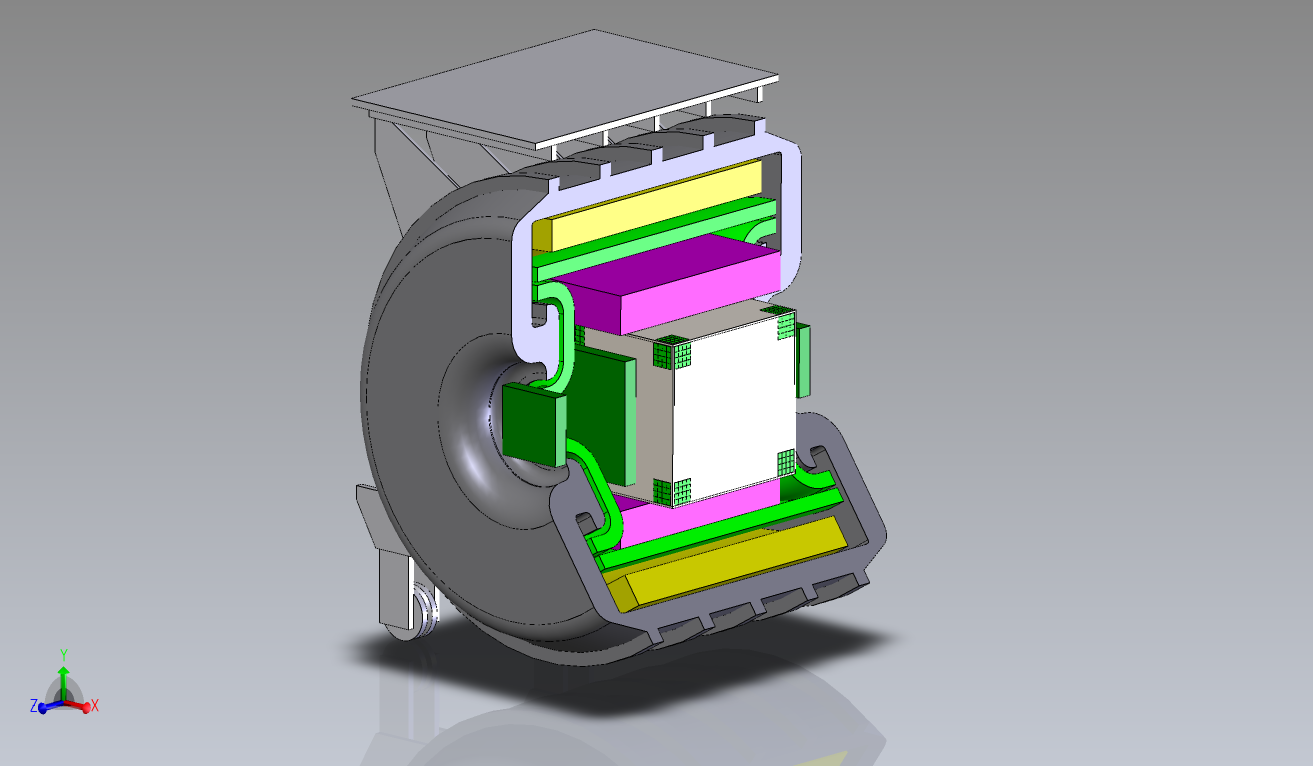
\includegraphics[width=7.in]{graphics/3DST-KLOE2019-08-01.png}
\end{dunefigure}




In addition, the \dword{3dst} has very fast timing and can isolate small energy depositions from neutrons in three dimensions.  This provides the capability to  incorporate neutrons in the event reconstruction using energy determination via time-of-flight with a high efficiency. This capability should be useful for the low-$\nu$ flux determination because it allows events to be tagged with a significant neutron energy component or provides a way to include that energy in the calculation.  Including neutrons in detailed studies of neutrino interactions in the \dword{3dsts} using single transverse variables may prove useful in motivating improvements in the neutrino interaction model. Although the target for this device is carbon, not argon, basic insights into components of the interaction model may extend to argon.  For example, the multinucleon component of the interaction model will be used for argon although it was developed in response to observations made on plastic targets.   



\section{Role of the ND in the DUNE Oscillation Program}
\label{sec:exsum-nd-role}

Oscillation experiments must accomplish three main tasks. First, they must identify the flavor of interacting neutrinos in \dword{cc} events or identify the events as \dword{nc} interactions. Second, they must measure the energy of the neutrinos because oscillations occur as a function of baseline length over neutrino energy, \dword{l/e}. Third, they must compare the observed event spectrum in the \dword{fd} to  predictions based on differing sets of oscillation parameters, subject to constraints from data observed in the \dword{nd}.  That comparison and how it varies with the oscillation parameters allows oscillation parameters to be measured.

The connection between the observations in the \dword{nd} and the \dword{fd} is made using a simulation that convolves models of the neutrino flux, neutrino interactions, nuclear effects, and detector response.
This gives rise to a host of complicating effects that 
muddy the simple picture. These complications come from two main sources. First, the identification efficiency is not \SI{100}{\%}, and there are
some background events (for example, \dword{nc} with a $\pi^0$ present %are 
a background to \nue \dword{cc} interactions). Both the efficiency and background are imperfectly known. %Generally, it is helpful to have a  \dword{nd} that is as similar as feasible to the  \dword{fd} because a bias in the efficiency as a function of energy will cancel between the two detectors. 
Because the background level tends to be similar in both the \dword{fd} and \dword{nd}, it helps if the \dword{nd} can characterize backgrounds better than the \dword{fd}. %, either due to its technology, or by leveraging the much larger statistics and freedom to take data in alternative beam configuration modes (for example, different horn currents or movement off the beam axis). 
%

The second major thing that complicates the simple picture is the \dword{fd} (and the similar \dword{nd}) must be made of heavy nuclei rather than hydrogen. %Neutrino interactions can be idealized as a three stage process: (1) a neutrino impinges on a nucleus with nucleons in some initial state configuration, (2) scattering occurs with one of the nucleons, perhaps creating mesons, and (3) the hadrons reinteract with the remnant nucleus on their way out (so called \dwords{fsi}). 
The presence of the nucleus affects %all three stages 
neutrino interactions in ways that ultimately drive the design of the  \dword{nd} complex. In particular, in a detector with heavy nuclei the nucleons in the initial state of the nucleus are mutually interacting and exhibiting Fermi motion. Neutrinos therefore interact with moving nucleon targets. The wavelength of the interaction varies with momentum transfer but is often long enough to simultaneously probe multiple nucleons. Another complication is that neutrino cross sections on {\em free nucleons} are not generally well known in the kinematic range interesting for \dword{dune}, but neutrino-nucleus scattering models rely on these neutrino-nucleus cross sections. A final complication comes about because neutrinos produce hadrons with the nucleus itself. After production the hadrons undergo \dword{fsi} and are thereby attenuated as they leave the target nucleus. Section~\ref{sec:appx-nd:exsum-nd-role} of Appendix~\ref{ch:appx-nd} discusses neutrino nucleus scattering in more detail. The \dword{dune} \dword{nd} includes liquid and gaseous active targets that will make high statistics measurements on argon, rather than another nucleus, to reduce nuclear model dependence. 


Neutrons can be produced from the struck nucleus, as well as from follow-on interactions of the neutrino's reaction-products with other nuclei. The energy carried away by neutrons is difficult to detect and can bias the reconstructed neutrino energy. The \dword{3dst} and \dword{mpd} have capabilities that allow neutron energy to be directly measured. The \dword{duneprism} program constrains the true to reconstructed energy relation and is thus also sensitive to energy carried by neutrons.

Heavy nuclei in the detector offer additional complications for particles that have left the struck nucleus, especially in the case where the detector is dense, as is the case for the \dword{lartpc}. Particles produced in a neutrino interaction may  reinteract inside the detector, creating electromagnetic and hadronic cascades. These cascades, particularly the hadronic ones, degrade the detector's performance. They confuse the reconstruction program due to overlapping energy and event features. They also result in a degredation of the energy resolution and result in additional energy carried by neutrons that may go missing. Particle identification by $dE/dx$ is also less effective for early showering particles. In addition, low-energy particle tracks in a dense detector may be too short to detect.  The \dword{dune} \dword{nd} includes the \dword{mpd} with a \dword{gartpc} that allows neutrino interactions to be measured on argon but with significantly fewer secondary interactions and much lower energy tracking thresholds.



Finally, setting aside complications due to heavy nuclei and dense detectors, we note that a significant fraction of the neutrino interactions in \dword{dune} will come from inelastic processes, not the simpler \dword{qe} scattering. 
This typically leads to a more complex morphology for events and greater challenges for the detector and the modeling.  The \dword{dune} \dword{nd} acts as a control for the \dword{fd} and is designed to be more capable than the \dword{fd} at measuring complicated inelastic events.

The complexity described above is incorporated imperfectly into the neutrino interaction model. The predicted signal in the \dword{nd} is a convolution of this interaction model with the beam model and the detector response model.  The critical role of  the  \dword{nd} is to supply the observations used to tune, or calibrate, this convolved model, thereby reducing the overall uncertainty in the expected signal at the \dword{fd} which is used for extracting the oscillation parameters via comparison with the observed signal.  Additionally, with the high statistics and very capable subsystems, the \dword{nd} data sets provide the raw material used to improve the models beyond simple tuning.  


%%%%%%%%%%%%%%%%%%%%%%%%%%%%%%%%%%%%%%%%%%%%%%%%%%%%%%%%%%%%%%
\section{ND Hall and Construction}
\label{sec:exsum-nd-hall}
%\input{vol-physics/nd-phys-from-LBNE-doc}

Figure~\ref{fig:es:NDhall} shows the current design of the underground hall required for the  \dword{nd} construction concept. The underground hall must house the detector components and allow required movement. The layout shows the space required for the detector, safety, and egress.  This  work is in progress. 


\begin{dunefigure}[DUNE near detector hall and detectors, plan view]{fig:es:NDhall}
{\dword{dune}  \dword{nd} hall shown from above (top) and from the side transverse to the beam (bottom). The \dword{lartpc}, \dword{mpd}, and \dword{3dst} detectors are shown in position on the beam axis in both drawings. }
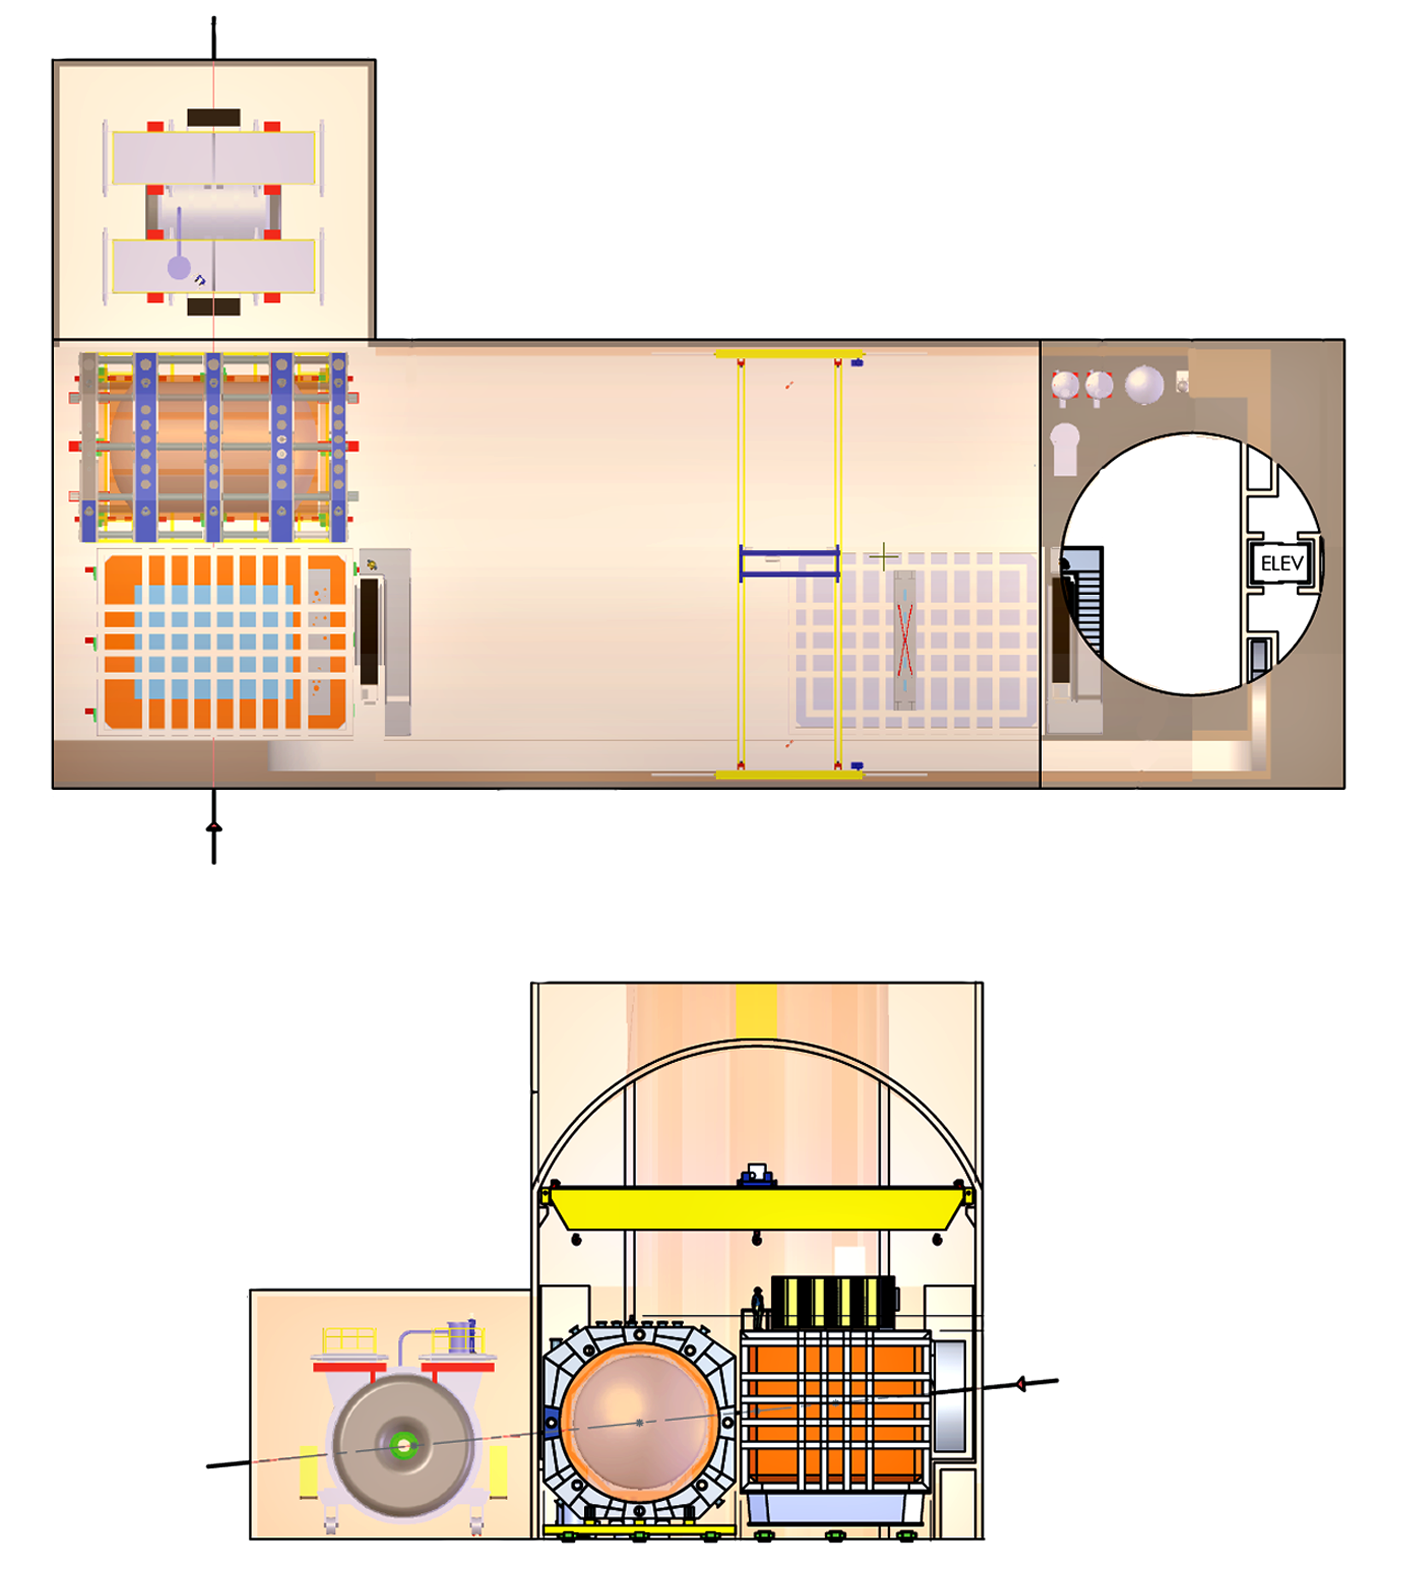
\includegraphics[width=0.8\textwidth]{nd-cavern-layout-no-dim}
%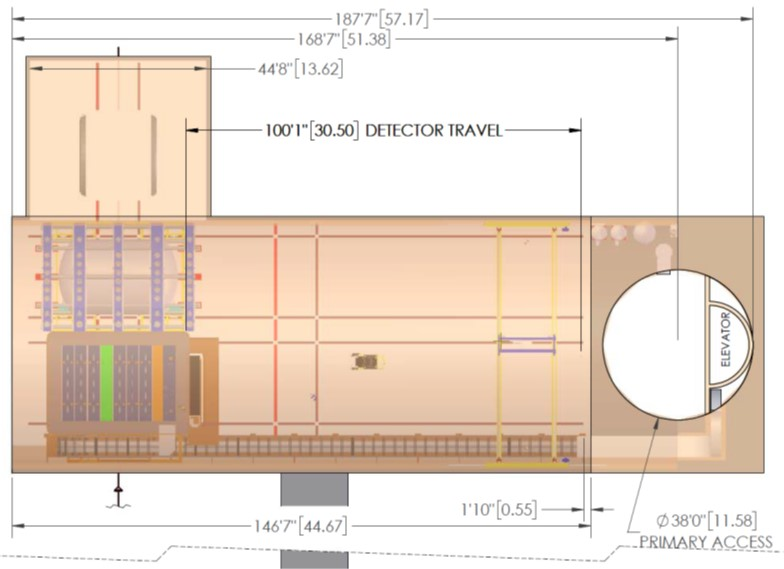
\includegraphics[width=0.8\textwidth]{graphics/Hall_top.jpg} replaced 11/6/19 from MLeitner
%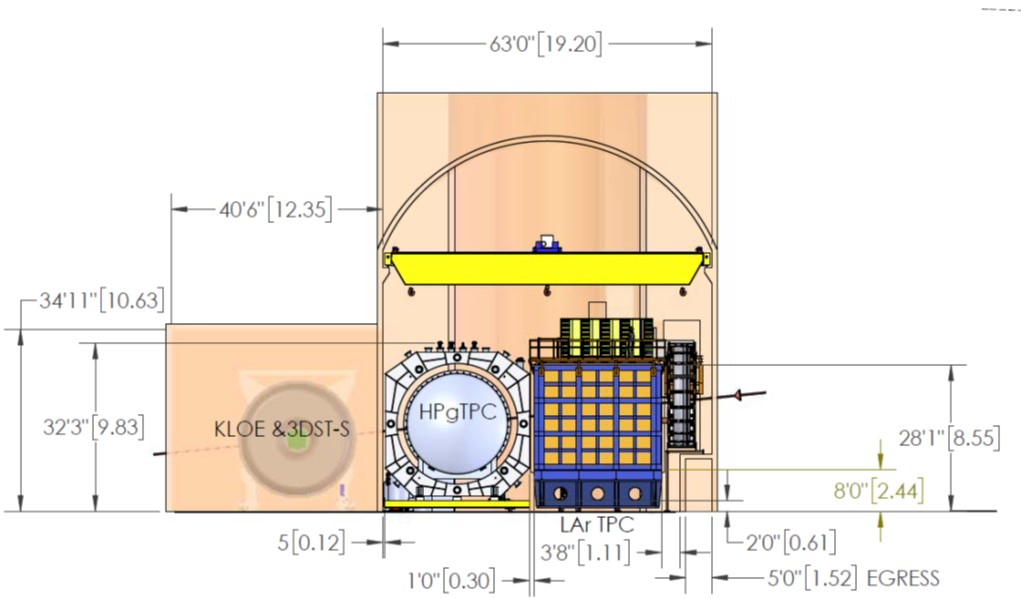
\includegraphics[width=0.8\textwidth]{graphics/Hall_side.jpg}
\end{dunefigure}

The overall construction method means the conventional facilities must meet certain requirements. 
The primary access shaft is large enough for lowering the pressure vessel and the magnet coils. The \dword{lar} cryostat is shown in its construction position near the main shaft. The \dword{mpd} and the \dword{lar} detector are also shown in the on-axis position. Because the \dword{3dst} detector does not need to move for \dword{duneprism}, it is shown in a dedicated alcove downstream of the \dword{lar} and multipurpose detectors.


The basic requirement for \dword{duneprism} is that both the \dword{mpd} and \dword{lar} detector can move horizontally to a position off the beam axis. The direction of the motion is to one side of the beam, and the total motion is approximately 30.5~m. 





